W celu utworzenia projektu koniecznym było wystawienie go dla osób trzecich, aby umozliwić testowanie przez osoby niezwiązane z pracą.
Domena jest to podstawowy inedytifkator tożsamości w internecie. Jest to element adresu internetowego aplikacji webowych.
Każdy może zakupić wolną domenę dla swoich celów. Należy w tym celu znaleźć odpowiadającego nam dostawcę i wykupić domenę o podanej nazwie.
Po tym procesie możemy bez problemu przekierować ją na żądany hosting lub też maszynę serwerową (rys. \ref{fig:domain}).

\begin{figure}[H]
    \centering
    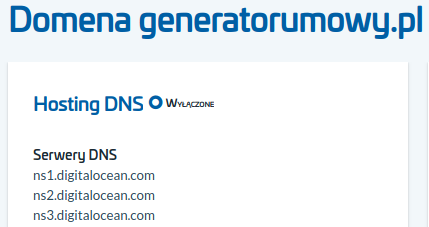
\includegraphics[width=6in]{images/domain.png}
    \caption{Przykładowa konfiguracja u dostawy az.pl \label{fig:domain}}
\end{figure}